\chapter{BugEnricher: Explaining Domain-specific Terms and Jargon from Bug Reports with Neural Machine Translation} \label{Chap2:BugEnricher}

\looseness=-1
Existing studies have shown that about 78\% of bug reports from open-source projects (e.g., Eclipse, Firefox) include less than 100 words each and claim more time from developers for bug resolution~\cite{zhang2017bug}. Our first study in Chapter \ref{chapter:BugMentor} aims to support the developers by generating answers to follow-up questions from deficient bug reports. While our answers have been found useful, novice developers might need more help in their bug understanding. In this chapter, we propose --- \textit{BugEnricher} --- that can supplement bug reports with meaningful explanations to their domain-specific terms or jargon. Our evaluation using three performance metrics (e.g., BLEU, METEOR, Semantic Similarity) shows that \textit{BugEnricher} can generate understandable and good explanations according to Google’s standard and can outperform existing baselines from the literature. \par

The rest of this chapter is organized as follows. Section~\ref{Chap2:Intro} introduces our study and reports the gap in the literature and our contribution. Section~\ref{Chap2:Motivation} illustrates the usefulness of our technique with a motivating example. Section~\ref{Chap2:Methodology} presents our proposed technique for explaining software-related terms. Section~\ref{Chap2:ExperimentalSetup} discusses our experimental design and datasets.
Section~\ref{Chap2:Results} discusses our evaluation results. Section~\ref{Chap2:RelatedWork} discusses relevant studies from the literature. Section~\ref{Chap2:Threats} identifies possible threats to the validity of our work. Finally, Section~\ref{Chap2:Summary} summarizes this study.


\section{Introduction} \label{Chap2:Intro}

Software bugs are human-made mistakes that prevent a software system from operating as expected.
According to a recent study~\cite{britton2013reversible, zou2018practitioners}, software bugs cause the global economy to suffer enormously and lose billions of dollars every year. Bug finding and corrections take up approximately 50\% of a developer's programming time. Bug resolution is, therefore, one of the most challenging issues in software maintenance~\cite{zou2018practitioners}. Hundreds of software bugs are submitted as \textit{bug reports} to bug-tracking systems such as GitHub and JIRA~\cite{anvik2006should}. The developers then examine and resolve these bugs by carefully analyzing the corresponding bug reports.

% motivation
Given a reported bug, developers need to first understand its root cause and symptom before they come up with a solution~\cite{bohme2017directed}. A recent study suggests that information in the majority of bug reports is incomplete and inaccurate~\cite{davies2014s,bugde2008global}. Zhang et al.~\cite{zhang2017bug} found that up to 78\% of bug reports from four open-source projects (e.g., Eclipse, Mozilla, Firefox, GCC) contain less than 100 words each (a.k.a., short bug reports). These short bug reports, on average, took 121 extra days to get resolved when compared to the well-written bug reports due to the lack of information~\cite{zhang2017bug}. Thus, understanding the bug reports could be a challenge due to incomplete or inaccurate information with complex problem context~\cite{velly2013towards}. This challenge could exacerbate for newcomers or novice developers to a project who need additional assistance to understand or resolve a bug. According to a recent study~\cite{guizani2021long}, even with prior experience, developers often need help to acquire a comprehensive understanding of any application domain and understand the discussions from a bug report. One significant obstacle to bug understanding for novice developers could be the lack of explanation for the domain-specific terms or jargon in the bug reports.\par

% why existing work is not sufficient
\looseness=-1
There have been existing studies to support newcomers or inexperienced developers who may struggle to comprehend the bug reports. An existing survey by Tan et al.~\cite{tan2020first} found that a clear bug description, which does not rely on in-depth domain knowledge, is crucial to assist newcomers in understanding and resolving the bug. Recently, Correa et al.~\cite{correa2013samekana} suggest that including web links in issue tracker discussions can benefit developers by providing external knowledge sources or artifacts. Zhang et al.~\cite{zhang2017bug} recommend complementing bug reports with carefully curated sentences from relevant past bug reports. Dit et al.~\cite{dit2008improving} propose a technique that suggests relevant comments from past bug reports so that developers can make explicit connections between the suggested and existing comments. Including such comments in a bug report can be helpful for the developers to gain a better understanding of the issue. While the above approaches offer complementary information to support bug understanding, they do not focus on domain-specific terms or jargon, which warrants further investigation.\par

% approach
\looseness=-1
In this chapter, we propose a novel technique --- BugEnricher --- that can supplement bug reports by generating explanations for their domain-specific terms and jargon using neural text generation. First,  we construct a vocabulary for two popular programming languages --- Java and Python. We scrape the domain-specific terms or jargon and their explanations from three different sources --- StackOverflow, Glossary, and API documentation. Second, we fine-tune a transformer-based text-generation model (e.g., T5) with the domain-specific terms or jargon and their corresponding explanations collected above. Third, we generate the explanations for domain-specific terms from bug reports using our fine-tuned model and examine their effectiveness using a case study.\par

\looseness=-1
We collect 28,7690 Java, 21,365 Python and 141,567 miscellaneous domain-specific terms or jargon and their explanations from the aforementioned sources for our experiments. We evaluate our technique --- BugEnricher --- using three popular metrics on text generation, namely BLEU score~\cite{papineni2002bleu}, METEOR~\cite{banerjee2005meteor}, Semantic Similarity Score~\cite{haque2022semantic}. We achieve a BLEU score of 28.85, which is understandable to good according to Google AutoML documentation~\cite{automldoc}. Our technique also outperforms two baselines --- AnswerBot~\cite{xu2017answerbot} and T5~\cite{raffel2020exploring} --- in all three metrics. We also conduct a case study using duplicate bug reports and attempt to enrich duplicate bug reports that are textually dissimilar~\cite{jahan2023towards}. We find that the enrichment of bug reports by BugEnricher led to an improvement in the performance of an existing technique for duplicate bug detection. Thus, the empirical findings above suggest that our technique has the potential to enrich a bug report significantly, which could lead to improved bug understanding and management.

% summary
We thus make the following contributions in this study:
\begin{enumerate}
    \item[(a)] A large dataset of 141,567 domain-specific terms and jargon and their corresponding explanations that are carefully curated from Stack Overflow Q\&A site, glossary, and API documentation.
    \item[(b)] A novel approach --- BugEnricher --- that can complement bug reports with meaningful explanations of their domain-specific terms or jargon using neural text generation (e.g., fine-tuned T5).
    \item[(c)] A replication package~\cite{bugenricherreplicationpackage} that includes our working prototype, experimental dataset, and other configuration details for the replication or third-party reuse.
\end{enumerate}    



\section{Motivating Example} \label{Chap2:Motivation}
% url  : https://bugs.eclipse.org/bugs/show_bug.cgi?id=440607
%  url : https://bugs.eclipse.org/bugs/show_bug.cgi?id=497389
\begin{figure}[!htpb]
  \centering
  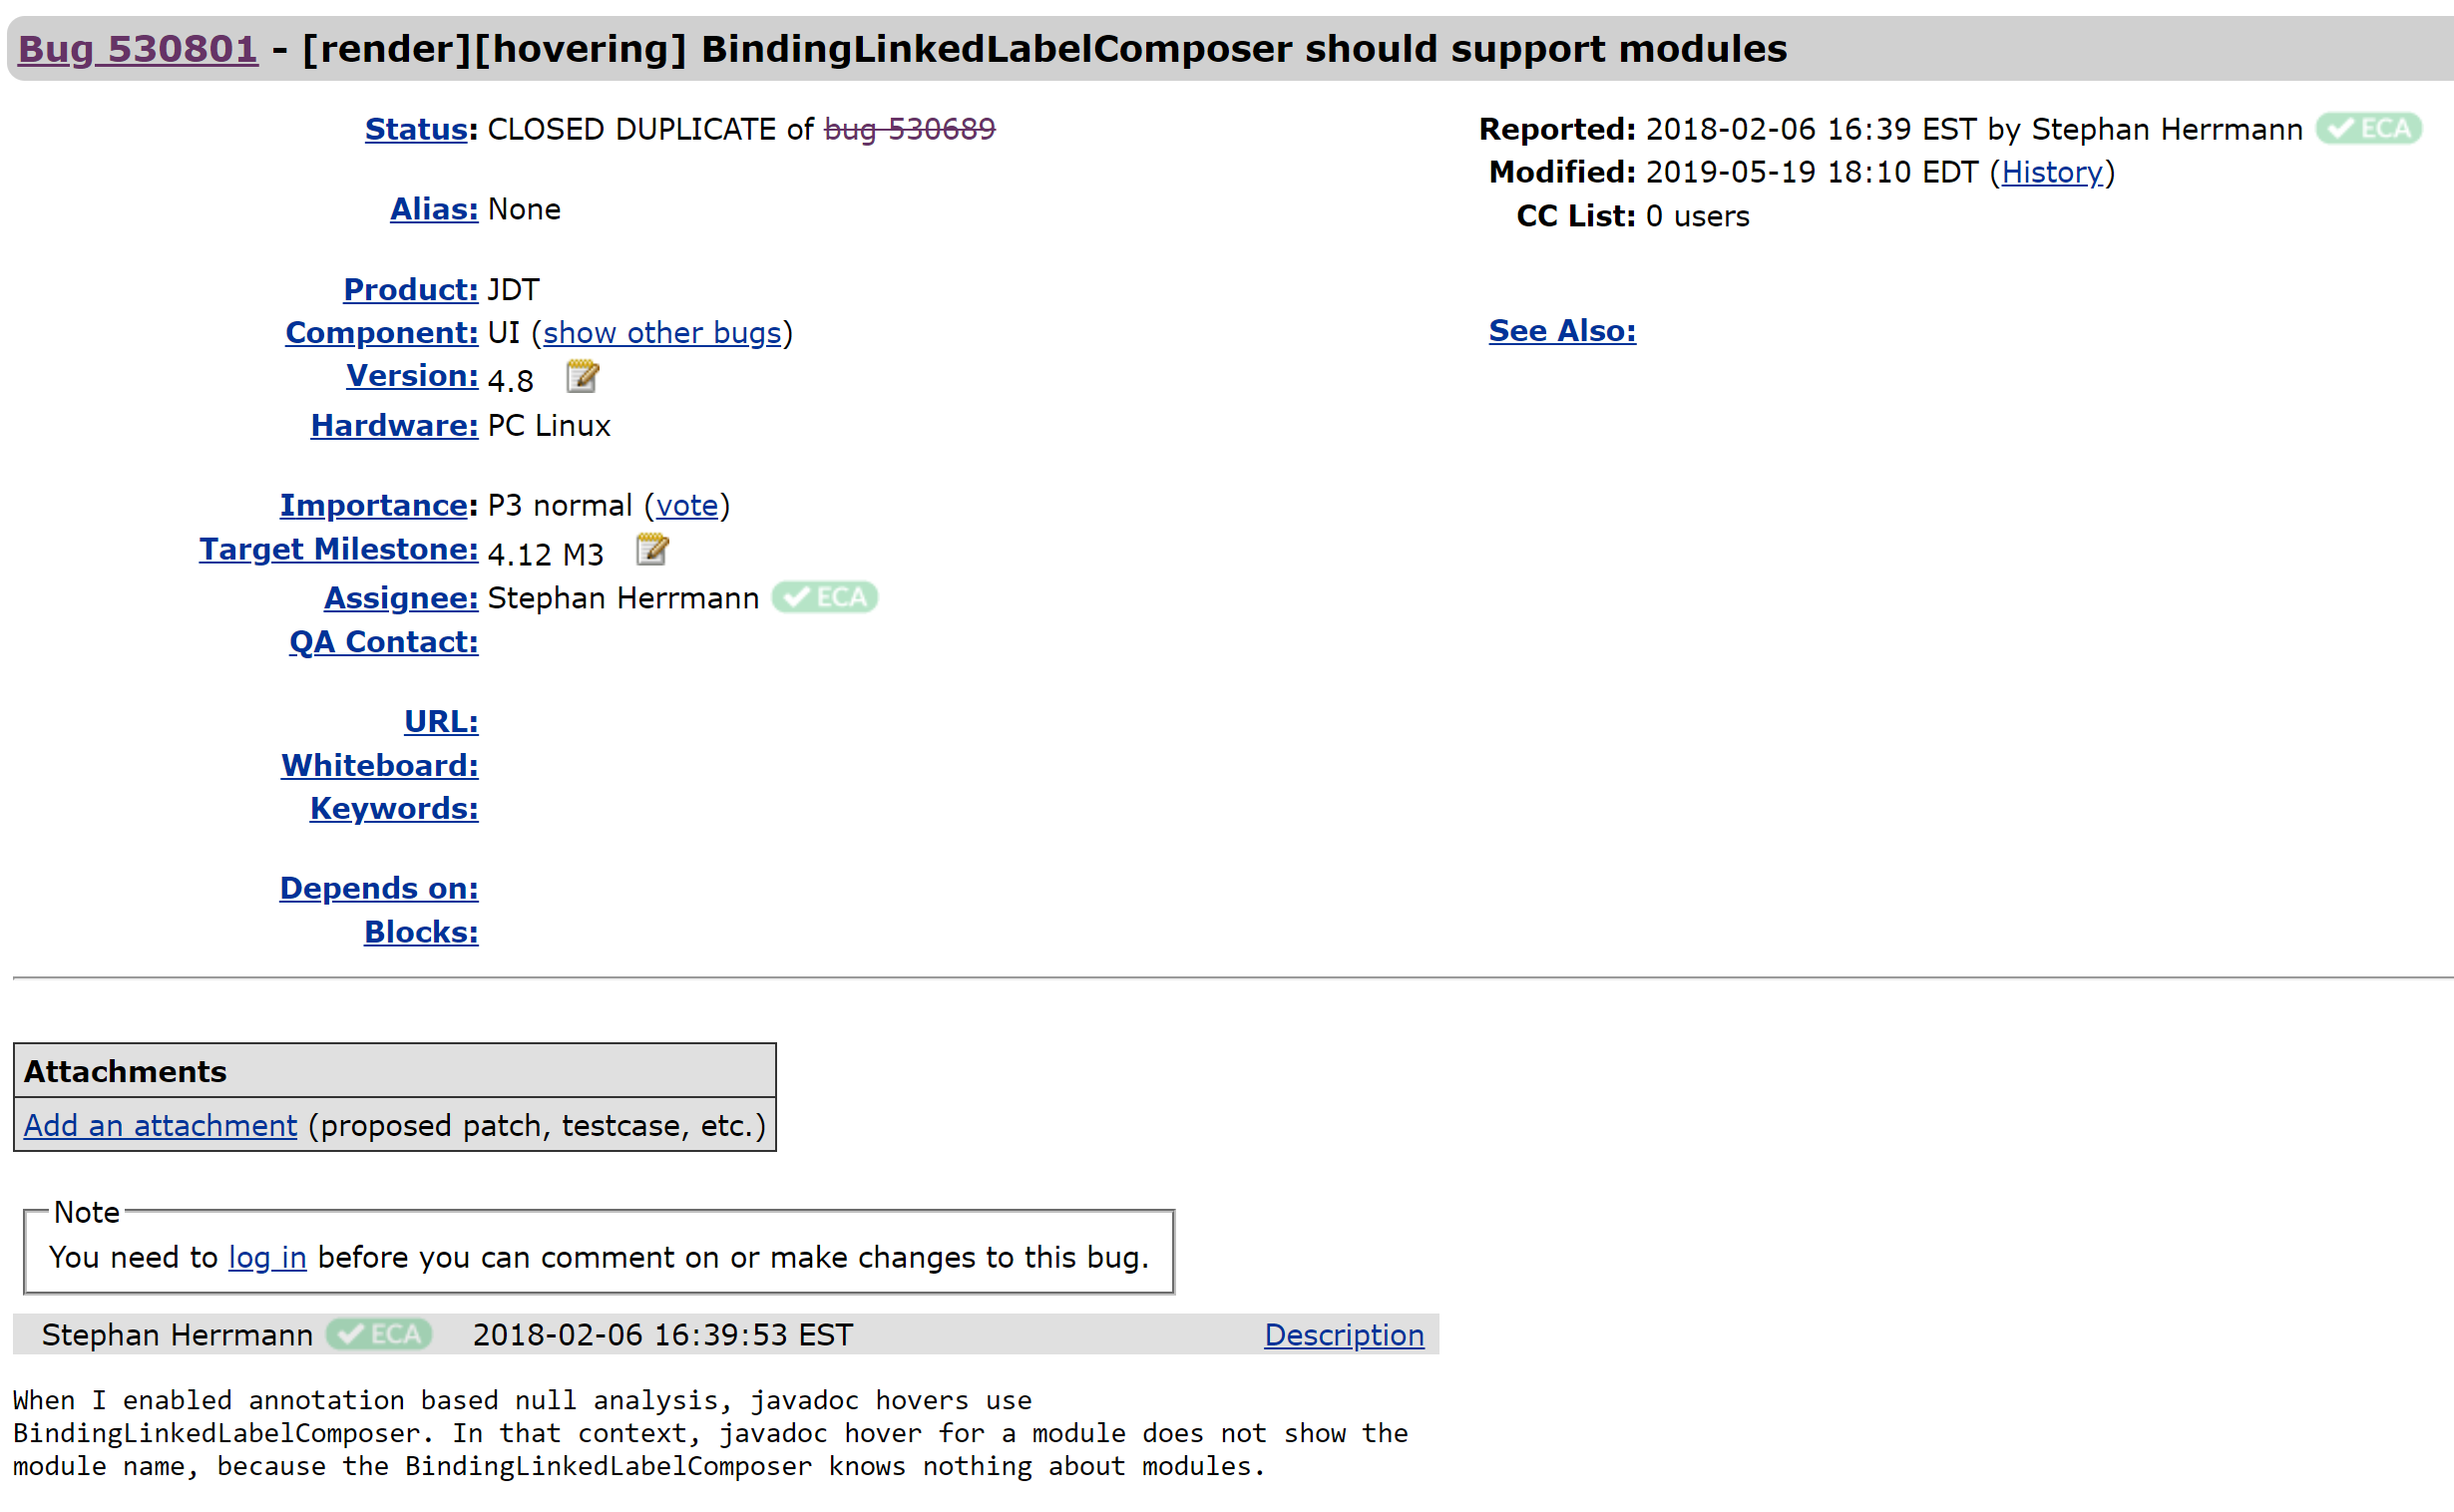
\includegraphics[width=0.9\textwidth]{images/motivatingexampleBE.png}
  \caption{An example of a bug report from BugZilla (ID \#530801)}
  \label{Chap2_fig:motivating_example}
\end{figure}

\begin{table}[!ht]
\centering
\caption{Generated Explanations by BugEnricher}
\label{BugEnricherGeneratedExplanations}
\resizebox{\textwidth}{!}{%
\begin{tabular}{|l|l|}
\hline
\textbf{Domain-Specific Terms or Jargon} & \textbf{Explanations} \\ \hline
Javadoc & It is documentation generated  \\ \hline
BindingLinkedLabelComposer & It is for composing labels \\ \hline
annotation & It is used to describe an annotation object \\ \hline
null-analysis & It is a Java library for analyzing null data \\ \hline
module & It is a unit of Java code \\ \hline
\end{tabular}%
}
\end{table}

\looseness=-1
To demonstrate the potential benefits of our work, let us consider the example bug report in Fig.~\ref{Chap2_fig:motivating_example}. It has been taken from the \emph{Eclipse} project on BugZilla\footnote{\url{https://bugs.eclipse.org/bugs/show_bug.cgi?id=530801}\label{chap2_motivating_example}}. The example report discusses a bug related to BindingLinkedLabelComposer that lacks awareness of modules. The problem stems from Javadoc when using the annotation-based null analysis. Specifically, the module name does not appear when hovering over a module. Table~\ref{BugEnricherGeneratedExplanations} shows the explanations generated by BugEnricher. These explanations were used to enrich the example bug report, and the enriched bug report can be found below.\par

\FrameSep.2em
\begin{frshaded}
\label{enrichedbugreport}
\noindent
 \textbf{Enriched Bug Report} \\
 \looseness=-1
When I enabled annotation (It is used to describe an annotation object) based null analysis (It is a Java library for analyzing null data), Javadoc (It is documentation generated) hovers use BindingLinkedLabelComposer (It is for composing labels). In that context, Javadoc hover for a module (It is a unit of Java code) does not show the module name, because the BindingLinkedLabelComposer knows nothing about modules.
\end{frshaded}

In our case study, the enriched bug report improved the rank of its duplicate report from the 19th to the 13th position in the ranked list when detected by a BM25-based technique~\cite{yang2012duplication,jahan2023towards}. This significant improvement in the ranking highlights the importance of our provided explanations, demonstrating an improvement in the quality of bug reports.

\section{Methodology} \label{Chap2:Methodology}

As input, our technique takes a bug report containing domain-specific terms or jargon that require additional explanation. As output, it generates explanations for those terms. Fig.~\ref{Chap2_fig:schematic} shows the schematic diagram of our proposed technique. In the following sections, we discuss different steps of our approach.\par 

\begin{figure}[!t]
  \centering
  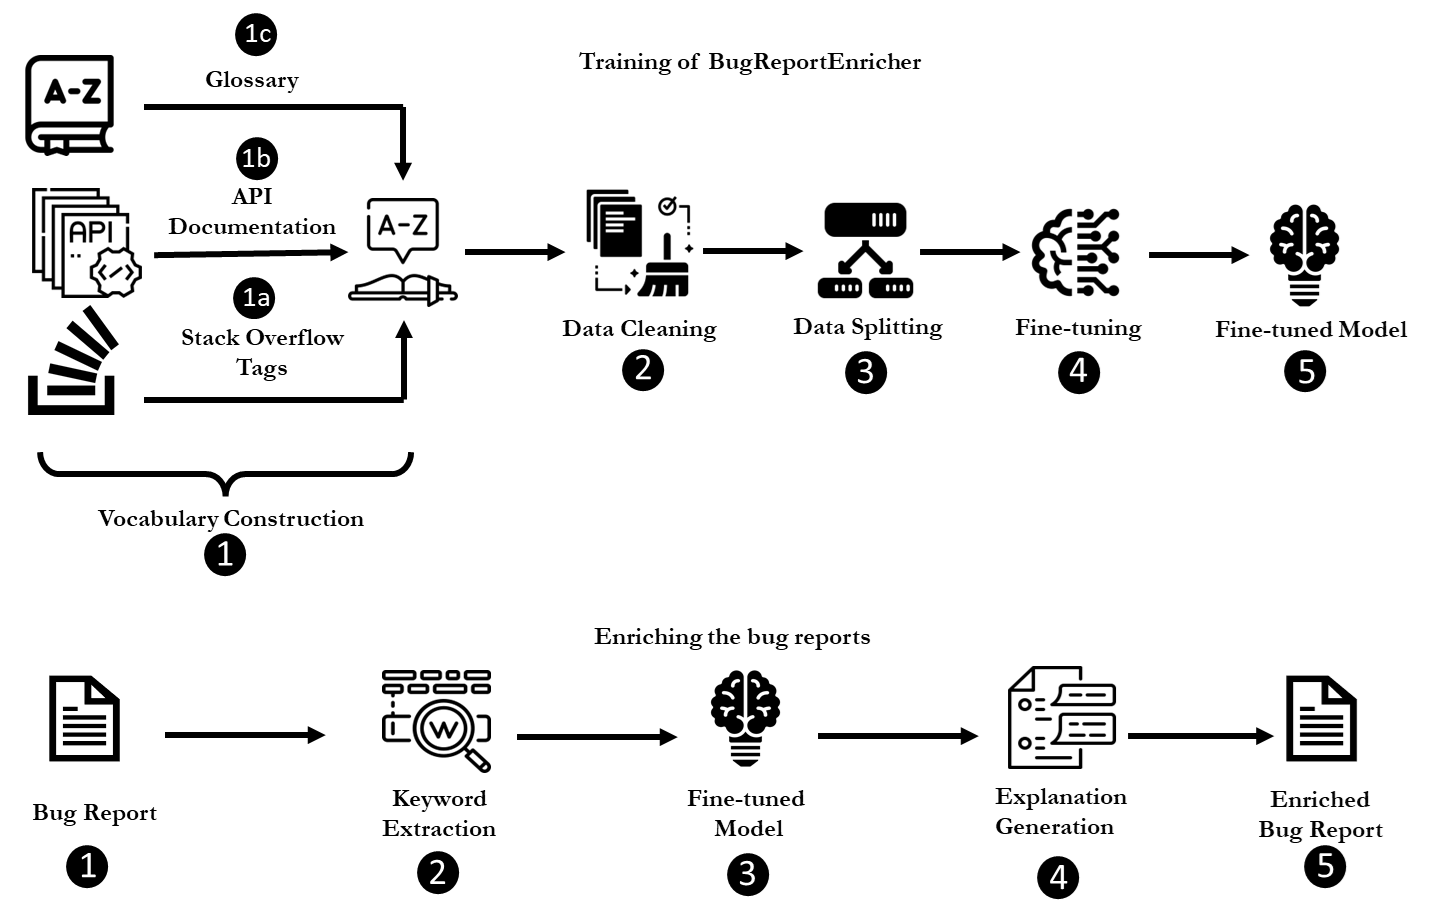
\includegraphics[ width=\textwidth, height=7.5in, keepaspectratio]{images/BugRepEnricherSchematic.png}
  \caption{Schematic diagram of BugEnricher}
  \label{Chap2_fig:schematic}
\end{figure}

\subsection{Vocabulary Construction}
First, we construct a vocabulary of domain-specific terms along with their meanings (a.k.a., explanations) for two popular programming languages --- Python and Java. We collect them from three different sources --- StackOverflow Tags, API Documentation and Glossary.

\subsubsection{(a) StackOverflow Tags}
To collect the domain-specific terms and their meanings, we use StackOverflow as our first source. Each post on StackOverflow consists of several tags that convey the key concepts of the post. The meaning of each tag is defined on StackOverflow. We collect 10,022 Java tags, 9,594 Python tags and 105,822 miscellaneous tags from \acrfull{sede} using the SQL query --- ``select $*$ TagName from Tags". The ``Tags" table contains all the name of the tags in the ``TagName" field. To capture the Java or Python related tags, we collect a list of Tags that contain the keyword ``Java" and ``Python" or "py" in their names. We then scrape the explanations of all the collected Tag names using Beautiful Soup\footnote{\url{https://pypi.org/project/beautifulsoup4/}}. An example of the StackOverflow tag is shown below.\par

\FrameSep.2em
\begin{frshaded}
\label{sotag}
\noindent
\textbf{Tag and Explanation at StackOverflow}\\
\textbf{Tag}: google-chrome-extension \\
\textbf{Explanation}: Extension development for the Google Chrome web browser. You write them using web technologies such as HTML, JavaScript, and CSS.
\end{frshaded}

\FrameSep.2em
\begin{frshaded}
\label{sotag2}
\noindent
\textbf{Java related Tag and Explanation at StackOverflow}\\
\textbf{Tag}: javafx-11 \\
\textbf{Explanation}: The JavaFX platform enables developers to create client applications based on JavaSE that behave consistently across multiple platforms. Built on Java technology since JavaFX 2.0, it was part of the default JDK since JDK 1.8, but starting Java 11, JavaFX is offered as a component separate from the core JDK.
\end{frshaded}

\FrameSep.2em
\begin{frshaded}
\label{sotag3}
\noindent
\textbf{Python related Tag and Explanation at StackOverflow}\\
\textbf{Tag}: python-mode \\
\looseness=-1
\textbf{Explanation}: Python-mode is a vim plugin that helps you to create Python code very quickly by utilizing libraries including pylint, rope, pydoc, pyflakes, pep8, and mccabe for features like static analysis, refactoring, folding, completion, documentation, and more.
\end{frshaded}

\looseness=-1
\subsubsection{(b) API Documentation}
We collect the API documentation of the most recent stable version of both Python (3.11) and Java (17) programming languages from their official documentation~\cite{pythonDocumentation,javaDocumentation}. We use Beautiful Soup\footnote{\url{https://pypi.org/project/beautifulsoup4/}} and Request\footnote{\url{https://pypi.org/project/requests/}} libraries for all our scraping.\par
First, we scrape the overview page from the official documentation containing the names of all the modules, their explanations and the URLs to further description of the defined packages and services. We store these module names and their explanations. Then, from the URLs collected in the previous step, we further scrape the package and service names, their explanations, and the URLs to further description of the defined classes and interfaces. Similarly, from the URLs collected in the previous step, we collect the classes and interfaces names, their explanations, and the URLs to the fields, methods and constructors names and their explanations. In total, we collect 18,738 Java and 11,771 Python terms and their explanations from the API documentation. An example of the terms and corresponding explanations from Java 17 and Python 3.11 API documentation is shown below.\par 

\FrameSep.2em
\begin{frshaded}
\label{apitagjava}
\noindent
\textbf{Term and Explanation from Java 17 API Documentation}\\
\textbf{java.io:} Provides for system input and output through data streams,
 serialization and the file system.\\
\textbf{java.lang:} Provides classes that are fundamental to the design of the Java
 programming language.
 \end{frshaded}

\FrameSep.2em
\begin{frshaded}
\label{apitagpython}
\noindent
\textbf{Term and Explanation from Python 3.11 API Documentation}\\
\textbf{str.splitlines:} Return a copy of the string with the leading and trailing characters removed.\\
\textbf{int.bit$\_$count:} Return the number of ones in the binary representation of the absolute value of the integer. This is also known as the population count.
 \end{frshaded}

\subsubsection{(c) Glossary}
As our third source, we collect 126 Java and 244 Python language-specific terms defined in the glossary. For Java we scrape from the oracle glossary \footnote{\url{https://www.oracle.com/java/technologies/glossary.html}\label{java-glossary}} and for python we scrape from the python glossary\footnote{\url{https://docs.python.org/3.11/glossary.html}\label{python-glossary}}.\par 
\FrameSep.2em
\begin{frshaded}
\label{glossarytag}
\noindent
\textbf{Term and Explanation from Java and Python Glossary}\\
\textbf{Python:} \\
\textbf{DOM:} Document Object Model. A tree of objects with interfaces for traversing the tree and writing an XML version of it, as defined by the W3C specification.\\
\textbf{Java:} \\ 
\textbf{immutable:} An object with a fixed value. Immutable objects include numbers, strings and tuples. Such an object cannot be altered.  A new object has to be created if a different value has to be stored.  They play an important role in places where a constant hash value is needed, for example, as a key in a dictionary.
 \end{frshaded}

After collecting the data from the three data sources, we discard any duplicates based on their terms and explanations. We divide the data into three different subsets --- Java, Python and Miscellaneous. The miscellaneous subset consists of terms and explanations from different programming languages. Table~\ref{tab:dataset} contains the descriptive statistics of our dataset. We find that the average length of each domain-specific term is approximately 13 characters, and their explanations have an average length of approximately 188 characters. \par

\renewcommand{\arraystretch}{1.4}
\begin{table}[htbp]
\centering
% \begin{threeparttable}
\caption{Dataset Details}
\label{tab:dataset}
\resizebox{\textwidth}{!}{%
\begin{tabular}{|c|c|c|c|c|c|}
    \hline
    \textbf{PL} & \textbf{Source} & \textbf{Size} & \begin{tabular}[c]{@{}c@{}}\textbf{ATL}\\ \textbf{(characters)}\end{tabular} & \begin{tabular}[c]{@{}c@{}}\textbf{AEL}\\ \textbf{(characters)}\end{tabular} & \textbf{Complete Size} \\ \hline \hline
    \multirow{3}{*}{Python} & Stack Overflow & 10,022 & 10.58 & 115.27 & \multirow{3}{*}{28,760} \\ \cline{2-5}
     & API Documentation & 18,738 & 16.72 & 360.10 &  \\ \cline{2-5}
     & Glossary & 126 & 14.31 & 361.40 &  \\ \hline
    \multirow{3}{*}{Java} & Stack Overflow & 9,594 & 11.88 & 121.38 & \multirow{3}{*}{21,365} \\ \cline{2-5}
     & API Documentation & 11,771 & 15.90 & 89.61 &  \\ \cline{2-5}
     & Glossary & 244 & 10.87 & 154.19 &  \\ \hline
    Micellaneous & Stack Overflow & 105,822 & 11.55 & 114.02 & 105,822 \\ \hline
    \end{tabular}
    }
    \vspace{-0.1cm}
\begin{threeparttable}
\begin{tablenotes}[flushleft]
  \small
  \item \begin{center}
      \item \textbf{PL} $=$ Programming Language, \textbf{ATL} $=$ Average Term Length,
      \item \textbf{AEL} $=$ Average Explanation Length
  \end{center} 
\end{tablenotes}
\end{threeparttable}
\end{table}

\subsection{Data Cleaning}
We use standard natural language pre-processing techniques to clean the domain-specific terms or jargon and their explanations. First, we remove the noisy elements like --- HTML tags and URLs. Second, we use the \textit{``pyspellchecker''}, a spell-checking library\footnote{\url{https://pypi.org/project/pyspellchecker/}\label{spellchecker}} to correct the spellings of any misspelled words. We then perform lemmatization on all items in our corpus. This step ensures that words are transformed into their root forms, facilitating better analysis~\cite{pramana2022systematic}.\par

\subsection{Data Splitting}
\label{Chap2:Methodology_datasplitting}

After we obtain the cleaned data from the previous step, we split each subset of terms and explanations into training, validation and test sets. We split each subset of our dataset (Java, Python, Miscellaneous) into training, validation and testing with the following ratios: 80\% training, 10\% validation, and 10\% testing data.

\subsection{Fine Tuning the Model}
\looseness=-1
\textbf{Model Input, Output and Structures:} 
We fine-tune the T5 model from HuggingFace\footnote{\url{https://huggingface.co/t5-base}} on the T5ForConditionalGeneration variant~\cite{huggingface_t5}, with our collected data. We use domain-specific terms or jargon as input (a.k.a., source sentence) and their explanations as output (a.k.a., target sentence). We train the T5 model with its associated encoder and tokenizer~\cite{raffel2020exploring}. The model has a 512-dimensional embedding size, a 6-layer encoder, and eight attention heads per layer. The model also has positional embeddings for sequences up to 512 tokens, contributing to its ability to handle diverse input lengths.

\textbf{Hyperparameter Tuning:} 
Applying grid search for hyper-parameter tuning is not feasible due to the large number of parameters in a T5 model (e.g., 60M to 220M parameters)~\cite{palivela2021optimization}. We thus perform heuristic-based hyperparameter tuning. We fine-tuned the T5 model through multiple iterations until it reached a stable BLEU score by tuning parameters such as learning rate, maximum sequence length, training batch size, and number of training epochs. We also repeat our training with ten random splits of the Java, Python and Miscellaneous datasets using scikit-learn's library~\cite{scikit} and report the average performance. We set the following parameters for our model training --- the train and valid batch sizes are both 8; the learning rate is $1e-4$; the maximum source and target text lengths are 128 and 512 tokens, respectively; and a random seed of 42 for reproducibility. Further details about the hyperparameters can be found in the replication package~\cite{bugenricherreplicationpackage}.

\textbf{Model Optimization and Regularization:} In configuring the model architecture, the feed-forward dimension is set to 2048, and dropout with a rate of 0.1 is applied for regularization. We also use the AdamW optimizer~\cite{loshchilov2017decoupled}, a variant of the Adam optimizer that corrects the weight decay regularization. The T5 model is trained on the Colossal Clean Crawled Corpus (C4), a large collection of approximately 750GB of English texts sourced from Common Crawl for text generation tasks. Thus, we did not pre-train it for our task since our dataset consists of natural language English language texts~\cite{raffel2020exploring}. \par

\looseness=-1
\textbf{Hardware Configuration and Training Time:} Our experiments are run on one NVidia A100 GPU with 40GB of memory. For the Java Dataset, the average model training time was approximately 30 hours, and the model was trained for 18 epochs. The average model training time for the Python dataset was approximately 30 hours, and the model was trained for 16 epochs. In the case of the Miscellaneous Dataset, a more extended training period is required. The average model training time for this dataset was approximately 120 hours, and the model is trained for 12 epochs.

% We use a batch size of 8 in each step. The average model training time for the Java and Python datasets is 30 hours for 18 and 16 epochs, respectively, and 120 hours for the miscellaneous dataset for 12 epochs.

\section{Experiment} \label{Chap2:ExperimentalSetup}
We evaluate our technique using three datasets containing domain-specific terms or jargon and their corresponding explanations using appropriate metrics from the relevant literature –-- \acrshort{BLEU} score~\cite{papineni2002bleu}, \acrfull{Semantic Similarity}~\cite{haque2022semantic}, and \acrshort{METEOR}~\cite{banerjee2005meteor}. Our datasets are based on Stack Overflow posts, API documentation, and glossary from two programming languages (Table~\ref{tab:dataset}). To place our work in the literature, we also compare our technique with two baseline techniques. Through our experiments, we answer three research questions as follows:
\begin{enumerate}
\item[(a)] \textbf{RQ$\mathbf{_1}$}: How does our technique perform in explaining domain-specific terms or jargon according to the automatic evaluation metrics?

\item[(b)] \textbf{RQ$\mathbf{_2}$}: Can our technique outperform the existing baseline techniques in generating explanations to domain-specific terms or jargon?

\item[(c)]\textbf{RQ$\mathbf{_3}$}: Does our enrichment of bug reports help improve an existing technique for duplicate bug report detection?
\end{enumerate}


\subsection{Dataset Construction}
To evaluate different aspects of our technique through experiments, we construct two datasets as follows:

\subsubsection{(a) Test Vocabulary} To answer RQ$\mathbf{_1}$ and RQ$\mathbf{_2}$, we reuse the dataset that we constructed earlier (Section~\ref{Chap2:Methodology}) and perform splitting to get 10\% testing data. Our test dataset contains 2,876 Java, 2,136 Python and 10,582 Miscellaneous terms and their explanations. We call them Java$_{TEST}$, Python$_{TEST}$, and Miscellaneous$_{TEST}$ respectively.

\subsubsection{(b) Bug Report Vocabulary} To answer RQ$\mathbf{_3}$, we collect 92,854 bug reports from an existing benchmark constructed from three open-source systems --- Eclipse, Firefox and Mobile~\cite{jahan2023towards}. We follow the approach of Jahan et al.~\cite{jahan2023towards} and apply standard natural language pre-processing techniques to each bug report. We discard stopwords since it does not capture any semantic meaning. We then split the bug report into tokens and remove noisy elements such as non-alphanumeric characters, numbers, HTML tags, and URLs. Lastly, we convert each bug report into lowercase text.

To obtain the infrequent, domain-specific terms or jargon from a bug report, we apply \acrshort{TF-IDF} based scoring to its content. We then collect the top 10 least frequent terms as domain-specific keywords from each bug report for explanation generation.

\subsection{Generating Explanations and Enriching Bug Report}\label{bugenricher:testdataset}
Using our fine-tuned T5 model, we generate the explanations for each of the domain-specific terms or jargon that are obtained from the previous step as follows. 

\subsubsection{(a) Test Vocabulary:} We generate an explanation for each term from all three datasets --- Java$_{TEST}$, Python$_{TEST}$, and Miscellaneous$_{TEST}$. We thus collect 2,876 Java, 2,136 Python and 10,582 Miscellaneous terms and generated explanations.

\subsubsection{(b) Bug Report Vocabulary:}
Using our fine-tuned model, we also generate explanations for the top 10 domain-specific terms or jargon from each bug report. The explanations are then injected into relevant places (see Section ~\ref{Chap2:Motivation}) within the texts to construct the enriched bug reports. We repeat this for all three subject systems --- Eclipse, Firefox and Mobile. We call these enriched bug reports --- Eclipse$_{Enriched}$, Firefox$_{Enriched}$ and Mobile$_{Enriched}$ and use them to answer RQ$\mathbf{_3}$. 

\subsection{Evaluation Metrics}
To evaluate the explanations from BugEnricher (a.k.a., fine-tuned T5 model) against the ground truth, we use three relevant metrics from literature --- BLEU Score~\cite{papineni2002bleu}, METEOR Score~\cite{banerjee2005meteor}, and Semantic Similarity metric~\cite{haque2022semantic}. They are defined as follows:

\subsubsection{\emph{\textit{BLEU --- Bi-Lingual Evaluation of Understudy} }}
BLEU score is a commonly used metric for evaluating translation~\cite{papineni2002bleu}, which has found application in many software engineering tasks (e.g., comment generation~\cite{hu2018deep}, text summarization~\cite{shi2022evaluation}). It compares a candidate text to a reference text and determines how similar they are based on the matching of their n-grams. The BLEU score is calculated as follows:
\begin{equation}
BLEU = BP \cdot exp \left ( \sum_{n=1}^{N}w_{n}log(p_{n}) \right )
\end{equation}
where $N$ is the maximum n-gram order, $w\textsubscript{n}$ is the weight assigned to the n-gram order, $BP$ is the brevity penalty --- a factor that penalizes the BLEU score when the candidate text is shorter than the reference text, and $p\textsubscript{n}$ is the modified n-gram precision, which measures the ratio of the overlapping n-grams (between the candidate text and the reference text), and the total number of n-grams in the candidate text.

\subsubsection{\emph{\textit{SS --- Semantic Similarity}}}
\looseness=-1
In a recent work, Haque et al.~\cite{haque2022semantic} investigate which metric best reflects human similarity assessment. They suggest that Sentence-BERT~\cite{reimers2019sentence} provides semantically meaningful sentence embeddings. Thus, when a candidate text is compared with the reference text based on these embeddings using cosine similarity, it has the highest correlation with human-evaluated similarity. The semantic similarity score is computed as follows:
\begin{equation}
SemSim(ref, gen) = \cos(\text{sbert}(ref), \text{sbert}(gen))  
\end{equation}
where $sbert(ref)$, and $sbert(gen)$ are the numerical representations from Sentence-BERT for the reference text and generated text, respectively.

\subsubsection{\emph{\textit{METEOR --- Metric for Evaluation of Translation with Explicit ORdering }}}
The \acrshort{METEOR} score is a metric for evaluating the quality of machine translation output based on both lexical and syntactic information~\cite{banerjee2005meteor}. It measures the similarity between a candidate text and the reference text by sequentially applying exact match, stemmed match and wordnet-based synonym match between the texts. 


\section{Evaluation of BugEnricher} \label{Chap2:Results}

\subsection{Answering RQ$\mathbf{_1}$ --- How does our technique perform in explaining domain-specific terms or jargon according to automatic evaluation metrics?} \label{Chap2:RQ1}

In this experiment, we analyze the performance of BugEnricher using three evaluation metrics - \acrshort{BLEU} score~\cite{papineni2002bleu}, \acrlong{Semantic Similarity} ~\cite{haque2022semantic} and \acrshort{METEOR} score~\cite{banerjee2005meteor}. We evaluate our fine-tuned model using a total of 15,594 domain-specific terms or jargon from three datasets --- Java$_{TEST}$, Python$_{TEST}$, and Miscellaneous$_{TEST}$ (Section~\ref{bugenricher:testdataset}). We collect explanations from BugEnricher for each of these terms and compare them against the ground truth explanations. Table~\ref{Tab:BugEnricherPerf} shows the performance details of BugEnricher. It should be noted that a higher value for \acrshort{BLEU}, \acrshort{METEOR}, and \acrlong{Semantic Similarity} is desirable in our experiments. \par

\looseness=-1
BugEnricher achieves a maximum \acrshort{BLEU} score of 28.85 for Java and 24.63 for Python, which are considered \textit{understandable to good} according to Google’s AutoML Translation documentation~\cite{automldoc}. This shows that the explanations from our model have a significant overlap with the ground truth in terms of individual words and phrases. However, the \acrshort{BLEU} score emphasizes capturing the precision of a response against the ground truth. Thus, we also evaluate our answers using the \acrshort{METEOR} score, which takes into account additional information such as synonyms, word forms, and sentence structure when capturing recall~\cite{banerjee2005meteor}.\par

\looseness=-1
In Table~\ref{Tab:BugEnricherPerf}, we find that our model achieves a maximum \acrshort{METEOR} score of 0.27 for Java and 0.23 for Python. This shows that BugEnricher was able to produce a significant part of the ground truth texts in its generated explanations. However, since \acrshort{BLEU} and \acrshort{METEOR} scores rely on keyword matching between a generated explanation and the ground truth explanation, they may not capture the semantic relevance between them. Hence, we also evaluate our generated explanations using \acrfull{Semantic Similarity} metric. Explanations from BugEnricher achieve a maximum of 53.26\% \acrfull{Semantic Similarity} for Java and 48.85\% for Python, which indicates a major semantic overlap with the ground truth explanations.

\renewcommand{\arraystretch}{1.1}
\begin{table}[!t]
\centering
\caption{Performance of BugEnricher}
\label{Tab:BugEnricherPerf}
\resizebox{0.7\textwidth}{!}{%
\begin{tabular}{|c|c|c|c|}
\hline
\textbf{Model} & \textbf{BLEU} & \textbf{METEOR} & \textbf{SS} \\ \hline \hline
\begin{tabular}[c]{@{}c@{}}BugEnricher$_{Python}$\end{tabular} & 24.63 & 0.23 & 48.85 \\ \hline
\begin{tabular}[c]{@{}c@{}}BugEnricher$_{Java}$\end{tabular} & 28.85 & 0.27 & 53.26 \\ \hline
\begin{tabular}[c]{@{}c@{}}BugEnricher$_{Miscellaneous}$\end{tabular} & 24.27 & 0.18 & 41.57 \\ \hline
\end{tabular}}
\end{table}

In Table~\ref{Tab:BugEnricherPerf}, we also report the performance of BugEnricher in cross-language settings (a.k.a, BugEnricher$_{Miscellaneous}$) where the domain terms or jargon are related to multiple programming languages and general software engineering. The goal was to determine the generality of our technique. We collect an explanation for each term from the Miscellaneous$_{TEST}$ dataset that contains 10,522 domain-specific terms or jargon and compare them against the ground truth explanation. We find that BugEnricher achieves a maximum \acrshort{BLEU} score of 24.27, \acrshort{METEOR} of 0.18 and \acrfull{Semantic Similarity} of 41.57\%. This shows that the generated and ground truth explanations are semantically and contextually similar even with this dataset. Despite the performance drop, BugEnricher can offer reasonable explanations across different programming languages, which is promising.\par

\FrameSep.3em
\begin{frshaded}
	\noindent
	\textbf{Summary of RQ$\mathbf{_1}$:} BugEnricher can generate meaningful explanations for domain-specific terms or jargon in Python and Java. The generated explanations are \textit{understandable} to \textit{good} according to Google's Standard, and they achieve a maximum BLEU score of 28.85, METEOR score of 0.27 and Semantic Similarity score of 53.26, which are promising.
\end{frshaded}


\subsection{Answering RQ$\mathbf{_2}$ --- Can our technique outperform the existing baseline techniques in generating explanations to domain-specific terms or jargon?}\label{Chap2:RQ2}

In this experiment, we compare our technique with two existing baselines in terms of evaluation metrics. To the best of our knowledge, there exists no work that automatically generates relevant explanations against domain-specific terms or jargon from a bug report. However, two existing question-answering techniques could be closely relevant to ours. AnswerBot~\cite{xu2017answerbot} can synthesize answers for Java-related technical, non-factoid questions from StackOverflow. T5~\cite{raffel2020exploring} is an encoder-decoder model trained on a large natural language corpus and has found numerous applications, including Question Answering. We thus consider these two techniques as our baselines for the comparison. We call them Baseline$_{AnswerBot}$, and Baseline$_{T5}$ respectively. Table~\ref{Chap2:Tab-baseline} shows the comparison details between BugEnricher and these baselines.\par


To implement Baseline$_{AnswerBot}$, we use the replication package provided by the authors~\cite{xu2017answerbot, maxxbw54}. To adapt it to our task, we append ``What is" as a prefix to each domain-specific term in the Java$_{TEST}$ dataset (Section~\ref{bugenricher:testdataset}) to construct the question. We use the author-provided corpus to capture answers (a.k.a., explanations) from this baseline. We observe that Baseline$_{AnswerBot}$ performs significantly poorly compared to BugEnricher but performs better than Baseline$_{T5}$. For example, Baseline$_{AnswerBot}$ achieves a maximum BLEU score of 15.23, METEOR score of 0.16 and Semantic Similarity of 32.47, which are lower than the corresponding measures of BugEnricher. BugEnricher achieves an overall performance gain~\cite{wattanakriengkrai2020predicting} of 72.12\%  across all three metrics compared to Baseline$_{AnswerBot}$.

\renewcommand{\arraystretch}{1.2}
\begin{table}[!t]
\centering
\caption{Baseline Performances}
\resizebox{0.5\textwidth}{!}
\end{table}

To implement  Baseline$_{T5}$, we use the T5-base model on HuggingFace~\cite{huggingface_t5}. We provide the model with the domain-specific terms from the Java$_{TEST}$ (Section~\ref{bugenricher:testdataset}) for our experiment. We use the T5ForConditionalGeneration implementation~\cite{huggingface_t5} of the baseline and capture explanations for each domain-specific terms or jargon. From Table~\ref{Chap2:Tab-baseline}, we observe that  Baseline$_{T5}$ performs poorly compared to Baseline$_{AnswerBot}$ and BugEnricher in generating explanations. For example, Baseline$_{T5}$ achieves a BLEU score of 10.62, a METEOR score of 0.13 and a Semantic Similarity of 27.89. This shows very limited contextual or semantic overlap between the generated explanation and the ground truth. Overall, BugEnricher achieves a performance gain~\cite{wattanakriengkrai2020predicting} of 88.34\% across all three metrics, compared to Baseline$_{T5}$.
% \vspace{-0.2cm}

\FrameSep.3em
\begin{frshaded}
	\noindent
	\textbf{Summary of RQ$\mathbf{_2}$:} BugEnricher performs better in generating explanations than both baselines in terms of three evaluation metrics. BugEnricher outperforms both baselines Baseline$_{T5}$ and Baseline$_{AnswerBot}$ by 72.12\% and 88.34\% respectively, across all three metrics.
\end{frshaded}

\subsection{ Case Study: Answering RQ$\mathbf{_3}$ --- Does our enrichment of bug reports help improve an existing technique for duplicate bug report detection?}\label{Chap2:RQ3}

Textually dissimilar duplicate bug reports differ from textually similar duplicate bug reports in terms of their underlying semantics and structures. For instance, textually dissimilar duplicate bug reports often have missing components (e.g., observed behaviours) or components that are written differently, which could lead to their overall textual differences~\cite{jahan2023towards}.\par

In this experiment, we examine whether our enrichment of bug reports with meaningful explanations can improve the detection of textually dissimilar but duplicate bug reports~\cite{jahan2023towards}. We use a popular IR-based technique --- BM25 --- to detect duplicate bug reports, as chosen by an existing work~\cite{jahan2023towards}. First, we extract the top ten infrequent terms from each bug report using TF-IDF (See Section~\ref{background:TF-IDF}). Then, we generate their explanations using BugEnricher and inject these explanations within the bug report. We call the datasets containing enriched bug reports --- Eclipse$_{Enriched}$, Firefox$_{Enriched}$ and Mobile$_{Enriched}$ in our experiment. Please check Section~\ref{Chap2:ExperimentalSetup} for further details on the experimental setup. We calculate, the Recall-rate@K of BM25 technique~\cite{yang2012duplication} performance metric for k = 1, 5, 10 and 100, as shown in Table~\ref{Table:EnrichedBugReports}.\par

We observe that the Recall-rate@K of the IR-based technique improves for the enriched bug reports across the three subject systems --- Eclipse$_{Enriched}$, Firefox$_{Enriched}$ and Mobile$_{Enriched}$. Interestingly, it performs better with Eclipse$_{Enriched}$ compared to Firefox$_{Enriched}$ and Mobile$_{Enriched}$. We also conduct the Mann-Whitney Wilcoxon test~\cite{cuzick1985wilcoxon} to check if the performance metrics with Eclipse$_{Enriched}$, Firefox$_{Enriched}$ and Mobile$_{Enriched}$ are significantly higher. We find that the performance improves by a statistically significant margin (p-value = 0.0004 $<$ 0.05). Thus, according to the above evidence, BugEnricher was able to offer complementary information to the bug reports through the explanations of domain-specific terms or jargon.

\renewcommand{\arraystretch}{1.6}
\begin{table}[!t]
\caption{Performance of a Duplicate Bug Report Detection technique using Enriched Bug Reports}
\label{Table:EnrichedBugReports}
\centering
\resizebox{0.8\textwidth}{!}{
\begin{tabularx}{\textwidth}{|>{\centering\arraybackslash}X|*{4}{>{\centering\arraybackslash}X|}}
\hline
\multicolumn{5}{|c|}{\textbf{BM25 for Duplicate Bug Report Detection}} \\ \hline
\multirow{2}{*}{\textbf{Dataset}} & \multicolumn{4}{c|}{\textbf{Textually Dissimilar Duplicates (Recall-rate@k)\%}} \\
\cline{2-5}
& \textbf{k=1} & \textbf{k=5} & \textbf{k=10} & \textbf{k=100} \\ \hline \hline
Eclipse & 21.83 & 37.5 & 41.27 & 52.58 \\ \hline
Eclipse$_{Enriched}$ & 28.16 & 40.24 & 44.94 & 56.17 \\ \hline
Firefox & 11.64 & 20.82 & 26.56 & 46.72 \\ \hline
Firefox$_{Enriched}$ & 15.47 & 21.05 & 26.71 & 49.63\\ \hline
Mobile & 15.73 & 28.09 & 35.96 & 59.55 \\ \hline
Mobile$_{Enriched}$ & 24.14 & 28.16 & 38.22 & 61.24 \\ \hline
\end{tabularx}}
\end{table}

\FrameSep.3em
\begin{frshaded}
	\noindent
	\textbf{Summary of RQ$\mathbf{_3}$:} BugEnricher is able to offer complementary information to textually dissimilar duplicate bug reports and enrich them through its explanations for domain-specific terms or jargon. These enriched bug reports were also found to improve the performance of an existing duplicate bug report detection technique by a statistically significant margin.
\end{frshaded}


\section{Related Work}\label{Chap2:RelatedWork}
\looseness=-1
Several existing studies attempt to help newcomers comprehend bug reports by complementing them with additional information. Correa et al.~\cite{correa2013samekana} proposed the inclusion of web links in issue tracker discussions that can benefit developers by providing external knowledge sources or artifacts. Zhang et al.~\cite{zhang2017bug} suggest enhancing bug reports with ranked sentences extracted from historical bug reports using information retrieval. Dit et al.~\cite{dit2008improving} introduce a technique that recommends relevant comments to help developers establish explicit connections between the recommended comments and existing comments. Moran et al.~\cite{moran2018enhancing} proposed FUSION, a tool for enhancing Android bug reports with reproduction steps of an Android bug. Mattia et al. ~\cite{fazzini2022enhancing} proposed EBUG that can provide a real-time understanding of reproduction steps in software bug reports. Xu et al.~\cite{xu2017answerbot} developed AnswerBot to generate responses for technical, non-factoid questions from StackOverflow. We compare BugEnricher with AnswerBot~\cite{xu2017answerbot} using experiments. The detailed comparison can be found in Section~\ref{Chap2:RQ2}.

In short, existing techniques provide additional information to complement bug reports through external resources and past relevant bug reports. However, they do not address the challenges novice or newcomer developers face in comprehending bug reports. To the best of our knowledge, our technique is the first to enrich bug reports with domain-specific terms or jargon explanations using neural text generation, which makes our work \textit{novel}. We found that the generated explanations from our technique outperform two existing baselines according to automated metrics. We also found that the enrichment of textually dissimilar bug reports with explanations for domain-specific terms or jargon improved the performance of an existing duplicate bug detection.

\section{Threats to Validity} \label{Chap2:Threats}
We identify a few threats to the validity of our findings. In this section, we examine these threats and discuss the steps that were taken to mitigate them.\par

\looseness=-1
\textbf{External Validity:}
Threats to external validity refer to the lack of generalizability in the findings~\cite{ferguson2004external}. One threat could stem from our selection of data sources. We select the API documentation and glossary of two programming languages and the Stack Overflow tags, which might not represent all relevant sources for software-specific terms or jargon. However, the underlying algorithm of BugEnricher is not bound to any programming language and thus can be easily adapted to any other data sources.\par 

\looseness=-1
\textbf{Construct Validity:} Construct validity refers to the extent to which the experiment measures what it intends to measure~\cite{smith2005construct}. 
Inappropriate use of evaluation metrics could be a threat to construct validity. However, we chose our evaluation metrics --- BLEU, METEOR, and Semantic Similarity --- based on relevant literature~\cite{papineni2002bleu,banerjee2005meteor,haque2022semantic,huang2016supervised}. Thus, threats to construct validity might be mitigated.\par

\looseness=-1
\textbf{Internal Validity:}
Threats to internal validity relate to experimental errors and subjective biases~\cite{christ2007experimental}. A source of threat could be the replication of the baseline techniques. For the replication of T5~\cite{raffel2020exploring}, we collected the pre-trained model from HuggingFace~\cite{huggingface_t5}. To replicate AnswerBot~\cite{xu2017answerbot}, we used the replication package from the original authors~\cite{maxxbw54}. Furthermore, we followed the documentation closely for any customizations. Thus, threats to internal validity might be mitigated.

\textbf{Limitation:} Our study contributes to explaining domain-specific terms or jargon that can be valuable to a developer in comprehending the bug report. However, it is essential to acknowledge certain limitations that may impact the generalizability and interpretation of the findings. Our selection of data could also introduce sampling bias. In future, we will consider more sources for domain-terms and jargon.\\
\textit{(a) Generalizability of Data:} In our study, we only use three different sources for collecting our data --- StackOverflow, Glossary and API documentation. However, they may not capture all domain-specific terms or jargon that could be present on a bug report.Our selection of data could also introduce sampling bias. In future, we will consider more sources for domain-terms and jargon.\\
\textit{(b) Dependency on Pre-trained Models:}
Our study utilizes pre-trained models such as T5 for generating explanations. The effectiveness of these models is contingent upon the quality and representativeness of the pre-training data. Issues such as biases present in the pre-trained models or their limited understanding of certain domain-specific nuances could impact the accuracy of explanations generated for bug reports.
\section{Summary} \label{Chap2:Summary}
Our previous study (Chapter 3) provides missing information to deficient bug reports by answering their follow-up questions. In this chapter, we propose BugEnricher that generates explanations to software-specific terms by learning from thousands of domain-specific terms and their explanations from Stack Overflow, official API documentation, and an online glossary. Our evaluation using three performance metrics shows that BugEnricher is able to generate understandable to good explanations to the domain-specific terms when compared against the ground truth as per Google's standards. Our technique was also able to outperform two existing baselines across three metrics. Furthermore, we also conduct a case study using duplicate bug reports and attempt to enrich duplicate bug reports that are textually dissimilar. We find that the enrichment of bug reports by BugEnricher improved the performance of an existing technique for duplicate bug detection. Thus, the empirical findings above suggest that our technique has the potential to enrich a bug report significantly, which could lead to improved bug understanding and management.